\documentclass[11pt, oneside]{article}
\usepackage[letterpaper, margin=2cm]{geometry}
\usepackage{AERE546}
\usepackage{xspace}
\newcommand{\xb}{\bar{x}}
\newcommand{\yb}{\bar{y}}

\begin{document}
\noindent \textbf{\Large{Caleb Logemann \\
AER E 546 Fluid Mechanics and Heat Transfer I \\
Homework 7
}}

%\lstinputlisting[language=MATLAB]{H01_23.m}
\begin{enumerate}
  \item % #1
    \begin{enumerate}
      \item[(a)]
        The following is my function that does Hermite Interpolation
        guaranteeing orthogonality at the walls.
        \lstinputlisting[language=MATLAB]{hermiteInterpolation.m}
    \end{enumerate}
      \begin{center}
        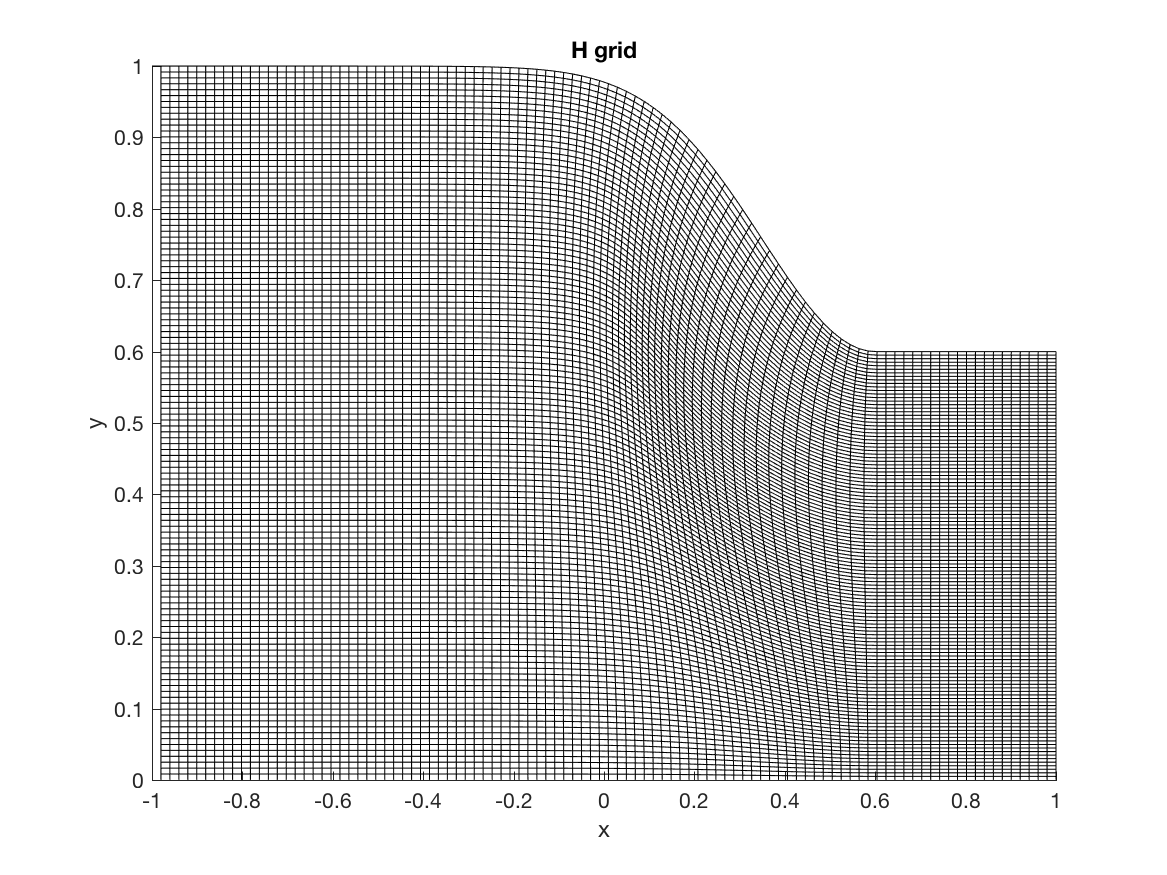
\includegraphics[scale=0.9]{Figures/07_01.png}
      \end{center}

    \begin{enumerate}
      \item[(b)]
        Again I use the hermiteInterpolation function from before.
    \end{enumerate}
      \begin{center}
        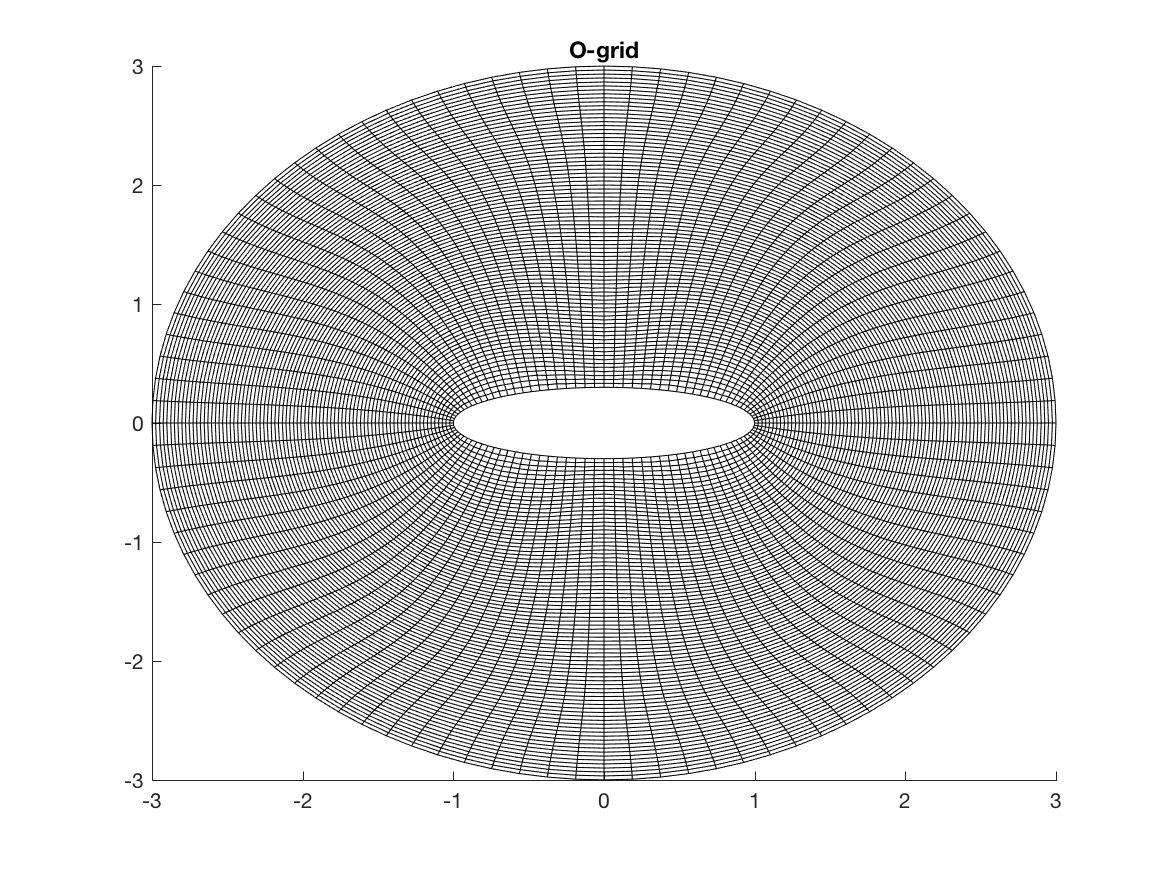
\includegraphics[scale=0.9]{Figures/07_02.png}
      \end{center}

    \begin{enumerate}
      \item[(c)]
    \end{enumerate}

  \item % #2

\end{enumerate}
\end{document}
